\documentclass{article}
\usepackage[T1]{fontenc}
\usepackage[margin=1in]{geometry}
\usepackage{graphicx}
\usepackage{float}
\usepackage{subcaption}
\usepackage{array}
\usepackage{xcolor}
\usepackage{hyperref}
\usepackage{listings}
\usepackage{caption}

\hypersetup{hidelinks}
\graphicspath{{report_assets/}}
\setlength{\parindent}{0pt}
\setlength{\parskip}{0.6em}

\title{\vspace{-2em}\centering ECE 111 TERM PROJECT PART 1}
\author{Anthony Villalino}
\date{21 March 2026}

\begin{document}
\maketitle

\section{ModelSim Verification}

The ModelSim screenshots show the completed Part 1 design running with no injected channel errors. In
\autoref{fig:modelsim-pass}, the top-level signals show \texttt{err\_inj = 00}, and the final scoreboard values
are \texttt{good = 256} and \texttt{bad = 0}. This is the clearest proof that the completed decoder works on
the provided testbench with error injection disabled.

\autoref{fig:modelsim-traceback} shows the decoder operating in steady state with \texttt{sample\_count},
\texttt{wr\_ptr}, and \texttt{traceback\_bit\_n} active. \autoref{fig:modelsim-metrics} provides a representative
view of the path metrics for the eight trellis states while the decoder is running.

\begin{figure}[H]
\centering
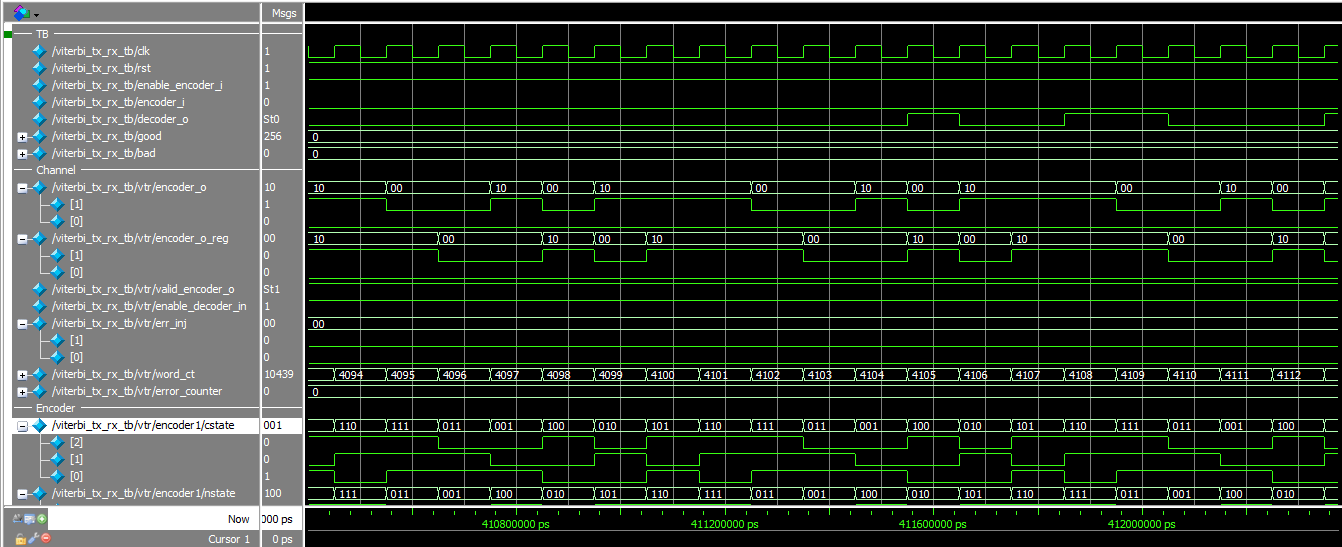
\includegraphics[width=\textwidth]{p1_waveform1.png}
\caption{ModelSim pass/fail proof. The no-error setting is active and the final
scoreboard shows \texttt{good = 256} and \texttt{bad = 0}.}
\label{fig:modelsim-pass}
\end{figure}

\begin{figure}[H]
\centering
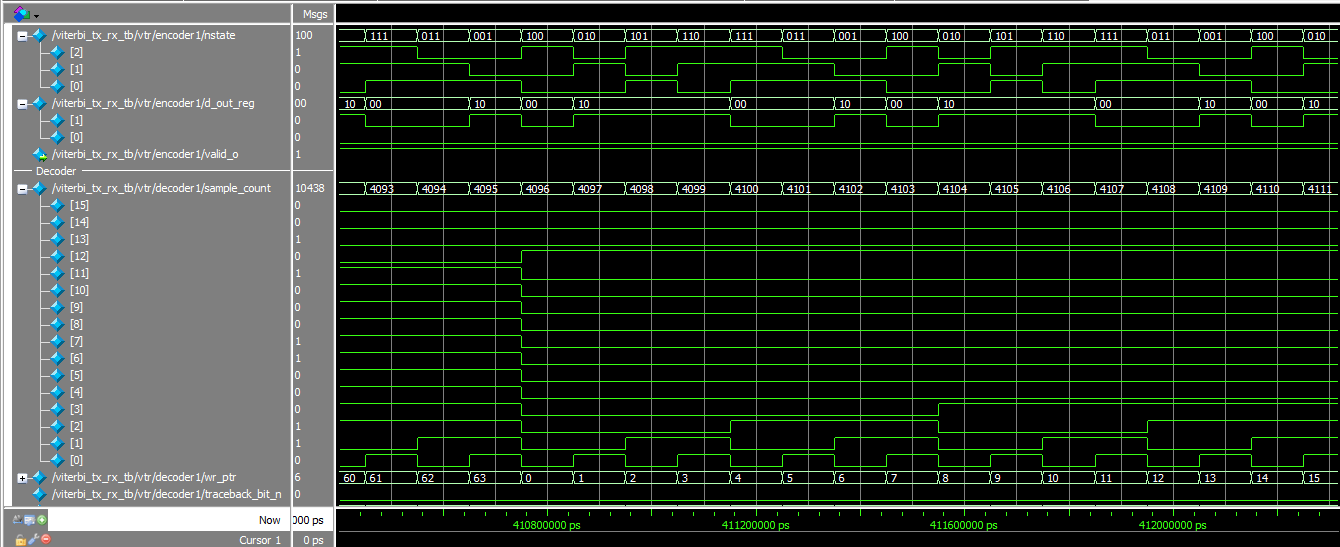
\includegraphics[width=\textwidth]{p1_waveform2.png}
\caption{Decoder activity. The screenshot shows
\texttt{sample\_count}, \texttt{wr\_ptr}, and \texttt{traceback\_bit\_n} during steady-state operation.}
\label{fig:modelsim-traceback}
\end{figure}

\begin{figure}[H]
\centering
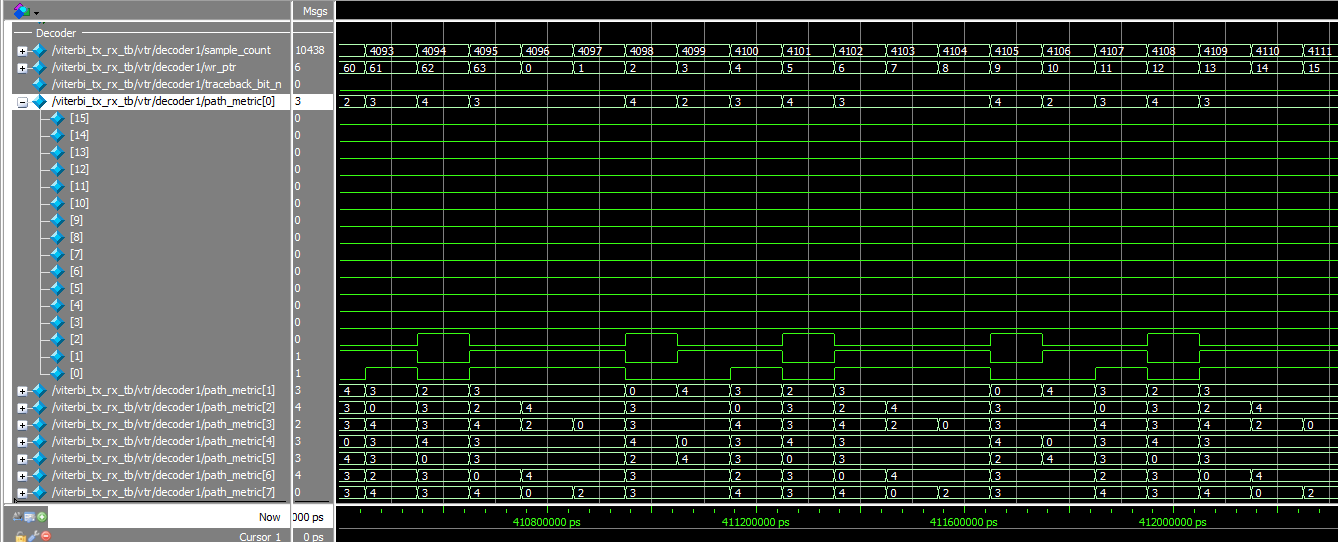
\includegraphics[width=\textwidth]{p1_waveform4.png}
\caption{Representative path-metric view. All eight decoder state metrics are
visible in one frame.}
\label{fig:modelsim-metrics}
\end{figure}

\section{Quartus Synthesis}

Quartus synthesis proof is shown by \autoref{fig:quartus-rtl} and the four resource-summary screenshots in
\autoref{fig:quartus-usage}. The RTL viewer screenshot shows the synthesized
top-level structure with the encoder block, the decoder block, and the pipeline registers between them.

\begin{figure}[H]
\centering
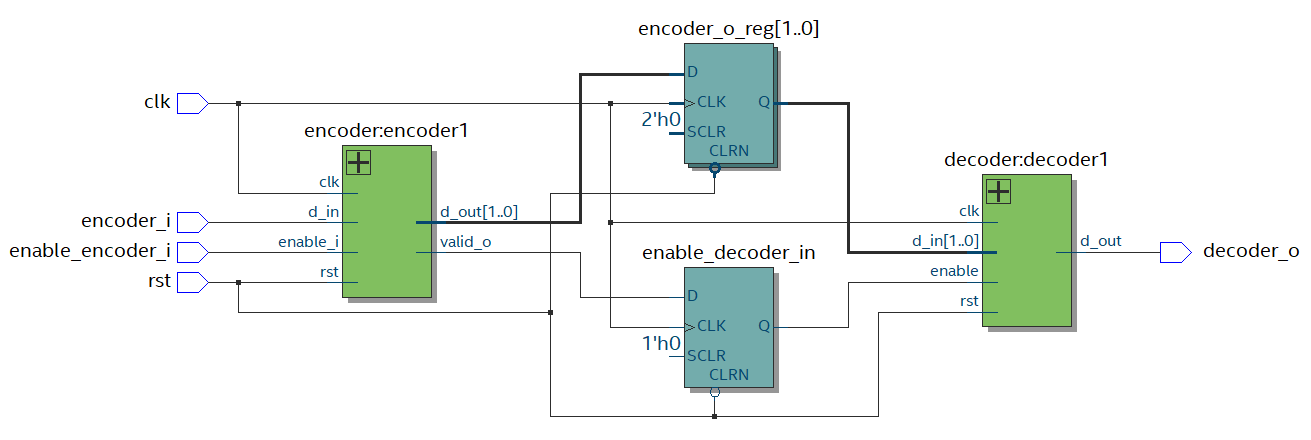
\includegraphics[width=\textwidth]{p1_RTL.png}
\caption{Quartus RTL viewer screenshot. The synthesized design contains the encoder,
registered channel interface, and decoder.}
\label{fig:quartus-rtl}
\end{figure}

The main utilization values visible in the Quartus screenshots are summarized below.

\begin{table}[H]
\centering
\caption{Quartus resource summary.}
\label{tab:quartus-summary}
\begin{tabular}{|>{\raggedright\arraybackslash}p{0.62\textwidth}|c|}
\hline
\textbf{Resource} & \textbf{Usage} \\
\hline
Estimated ALUTs used & 12,342 \\
\hline
Dedicated logic registers & 4,961 \\
\hline
Estimated ALUT/register pairs used & 24,682 \\
\hline
I/O pins & 5 \\
\hline
DSP block 18-bit elements & 0 \\
\hline
Maximum fan-out & 4,961 \\
\hline
Total fan-out & 89,408 \\
\hline
Average fan-out & 5.16 \\
\hline
7-input combinational functions & 128 \\
\hline
6-input combinational functions & 11,094 \\
\hline
5-input combinational functions & 136 \\
\hline
4-input combinational functions & 221 \\
\hline
\(\leq\)3-input combinational functions & 763 \\
\hline
Normal-mode ALUTs & 11,943 \\
\hline
Extended-LUT-mode ALUTs & 128 \\
\hline
Arithmetic-mode ALUTs & 271 \\
\hline
\end{tabular}
\end{table}

\begin{figure}[H]
\centering
\begin{subfigure}[t]{0.48\textwidth}
\centering
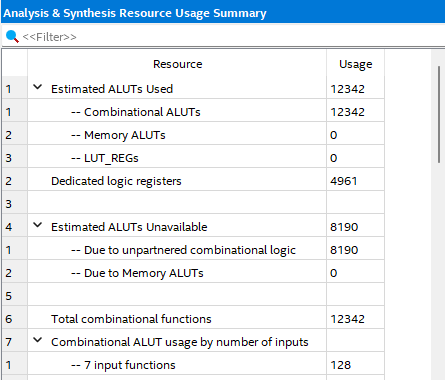
\includegraphics[width=\textwidth]{p1_usageSum1.png}
\caption{Resource summary view 1}
\end{subfigure}
\hfill
\begin{subfigure}[t]{0.48\textwidth}
\centering
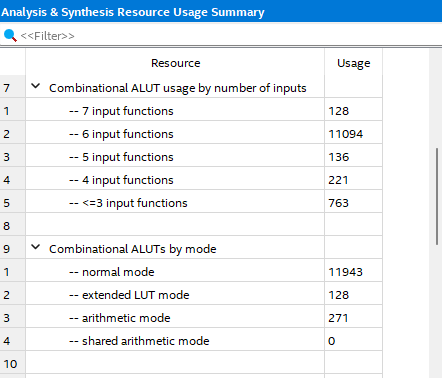
\includegraphics[width=\textwidth]{p1_usageSum2.png}
\caption{Resource summary view 2}
\end{subfigure}

\vspace{0.75em}

\begin{subfigure}[t]{0.48\textwidth}
\centering
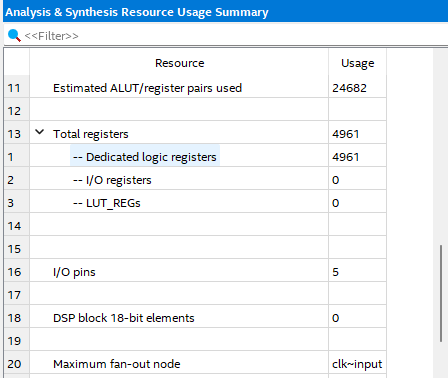
\includegraphics[width=\textwidth]{p1_usageSum3.png}
\caption{Resource summary view 3}
\end{subfigure}
\hfill
\begin{subfigure}[t]{0.48\textwidth}
\centering
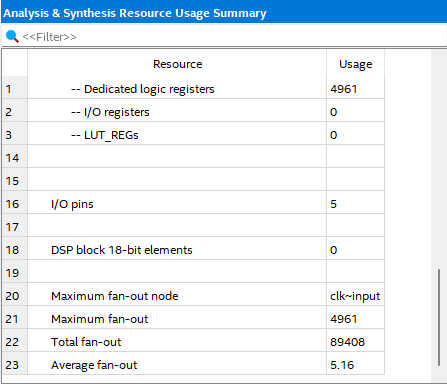
\includegraphics[width=\textwidth]{p1_usageSum4.png}
\caption{Resource summary view 4}
\end{subfigure}
\caption{Quartus Analysis and Synthesis Resource Usage Summary screenshots.}
\label{fig:quartus-usage}
\end{figure}

\section{Encoder}

The supplied encoder is not the same as the Homework 7 encoder, so it must be used with this decoder. Its
behavior is defined by the state and output equations in \texttt{encoder.sv}:

\[
\begin{array}{l}
d\_out[0] = d\_in \\
d\_out[1] = d\_in \oplus cstate[2] \oplus cstate[1] \\
nstate[1:0] = cstate[2:1] \\
nstate[2] = d\_in \oplus cstate[1] \oplus cstate[0]
\end{array}
\]

The first encoded bit is the input bit itself, while the second encoded bit is a parity bit formed from the
input and two state bits. The next state is also project-specific because the new MSB includes XOR feedback.
That exact output and state-transition rule defines the trellis that the decoder must follow.

\section{Decoder}

The decoder performs Viterbi decoding across 8 trellis states. For each next state, it compares the two possible
predecessor branches and keeps the branch with the lower accumulated cost. The branch metric is a two-bit Hamming
distance between the received symbol and the symbol predicted by the encoder model:

\[
\text{branch metric} = (r_1 \oplus e_1) + (r_0 \oplus e_0)
\]

With no errors present in Part 1, the correct branch matches the received symbol exactly, so both XOR terms are 0.
That is why the minimum branch metric is 0 when the channel is not corrupting the encoded data.

After the branch metrics are added to the previous path metrics, the decoder stores the winning predecessor for
each state. Once enough survivor history is available, it traces backward through those stored decisions and
outputs the bit associated with the lowest-cost trellis path. This is how the decoder determines what sequence
of bits was originally sent to the encoder.

\section{Conclusion}

The screenshot set provides the required Part 1 proof items. The ModelSim results show a passing run with
\texttt{good = 256}, \texttt{bad = 0}, and no channel error injection. The Quartus results show successful
synthesis, an RTL view of the design, and the device utilization summary.

\end{document}
